%! TEX root = ../aminhash.tex

\section{Introduction}
Quantization a key ingredient in modern search systems.
By reducing the space required by data, it not only allows is critical to storing the data at all, it also increases data locality allowing faster search and algorithms working on the quantized data.
%Reducing the space required to store data, it serves a double purpose of increasing data locality for faster search; and of actually allowing the data to be stored in the first place.

MinHash sketches (Min-wise sketches) are randomized summaries of sets (or equivalently $0/1$ vectors).
The idea is to pick $K$ random functions $h_i : U \to [0,1]$ and define the sketch of $X\subseteq U$ to be
$q(x) = (\argmin_{x\in X}h_1(x), \dots, \argmin_{x\in X}h_K(x))$.
% TODO: references
After early uses in statistics~\cite{brewer1972selecting} and correlation estimation~\cite{flajolet1985probabilistic}, the term was coined by Broder~\cite{broder1997resemblance} in the context of detecting near-duplicate web pages.

MinHash is particularly popular for searching genomes and metagenomes in Bioinformatics~\cite{ondov2016mash} and other large sparse categorical data.
A typical scenario is that we want to store some sets $Y_1, \dots$, so we compute the MinHash sketch for each of them, with perhaps $K=100$.
Now, given a new set, $X$, we hash it and estimate the similarity with each $Y_i$ by $\|q(X)-q(Y_i)\|_1/k$, which has expectation $\frac{|X\cap Y|}{|X\cup Y|}$, known as the Jaccard similarity between $X$ and $Y$.

Since $q(X)$ only has to be computed once, and east subsequent estimate takes time $K$, rather than $|X \cap Y|$, the quantized database can often be searched substantially faster than the naive approach.
Such quantization can be combined with space partition methods to produce state of the art set search, such as~\cite{christiani2018scalable}.

Quantization is similarly important in nearest neighbour search in Euclidean distance.
In their seminal paper, Jegou et al.~\cite{jegou2010product}
%recognized that compressed representations allow for faster search, even when the data is already dense in $\R^{100}$, say.
%This is mainly due to greater data locality and cache usage.
argued for the application of ``asymmetric distance estimation'' as a way to improve search accuracy and speed in this context.
Instead of sketching the query and computing the similarity ``in sketch-space'', $\|q(x)-q(y)\|_1$,
one can use the full information of the query and compute $\|x-q(y)\|_1$ with no loss in speed or memory efficiency.
see~\cref{fig:jegou} for a visualization.
%For example, a search engine may store sketches of billions of documents to be searched, but when a query arrives, there is no performance reason to sketch it.


\begin{figure}[h]
   \centering
   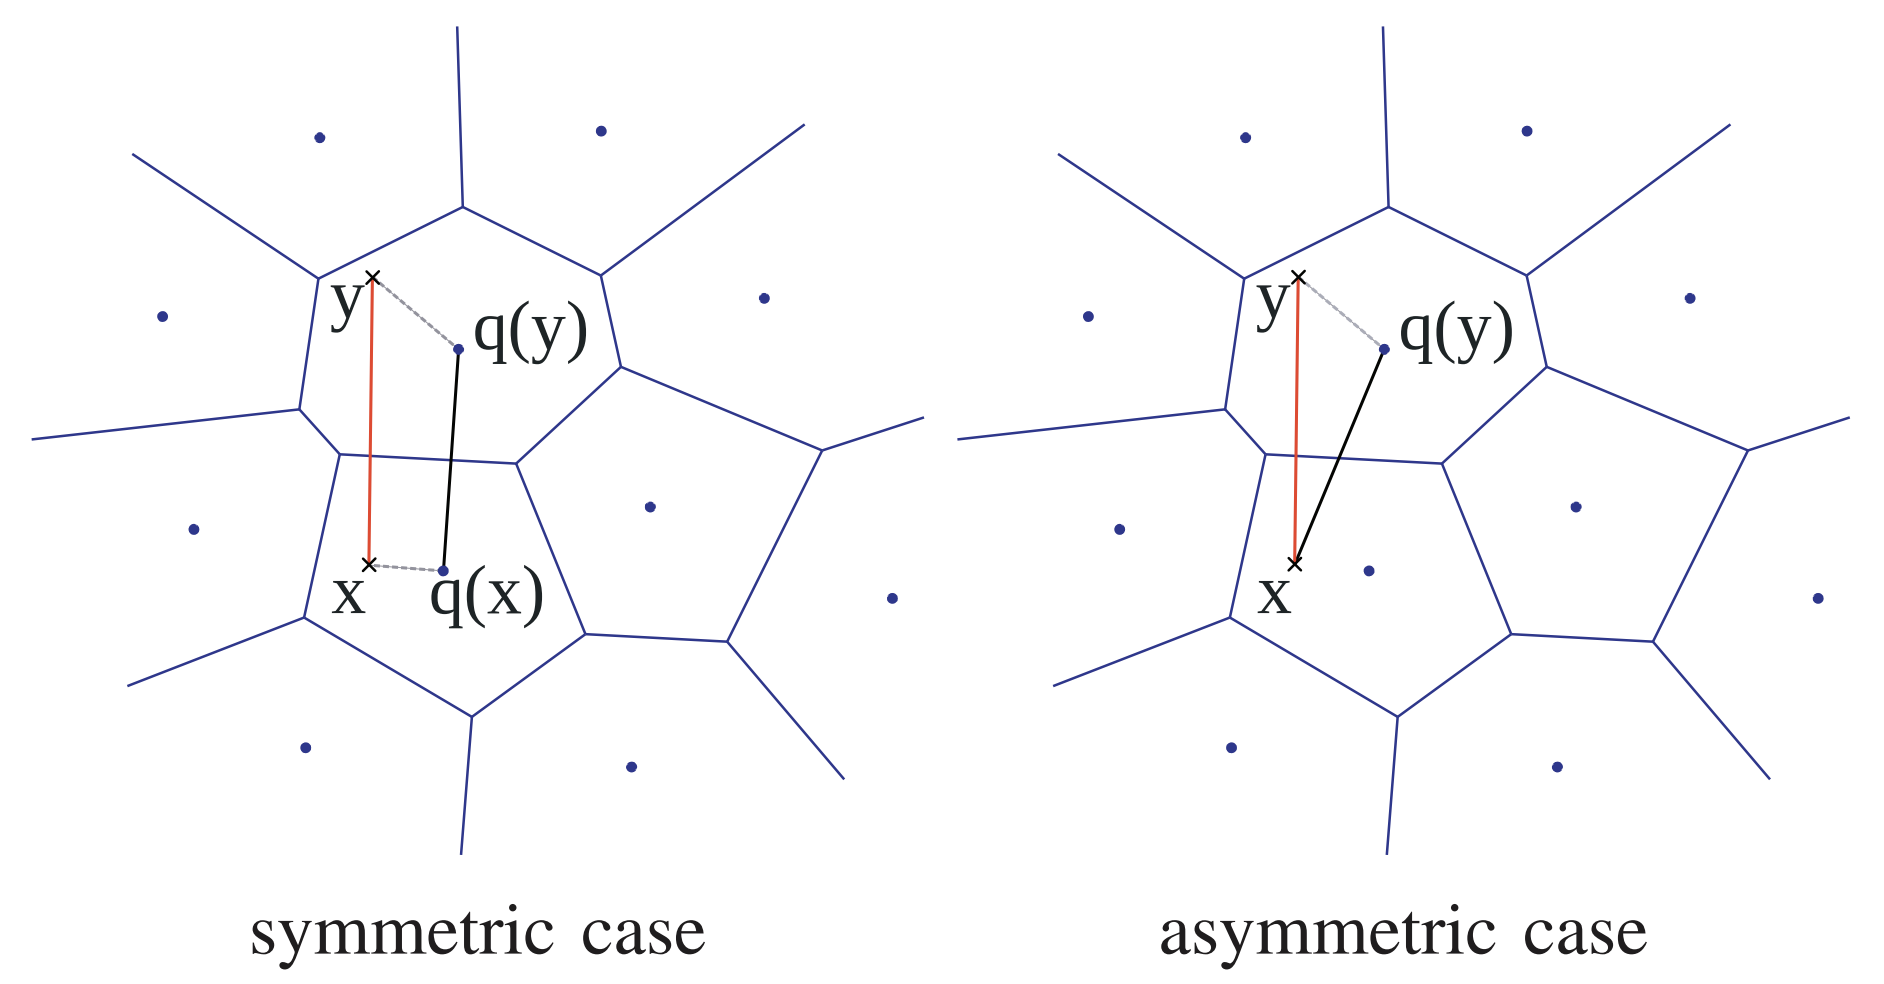
\includegraphics[width=\linewidth]{figures/pq}
\caption{Figure by Jegou et al.~\cite{jegou2010product} illustrating the difference between symmetric and asymmetric estimation, as used in Euclidean Nearest Neighbour Search.
   The distance $q(y)-x$ is a better approximation of $y-x$ than $q(y)-q(x)$.
   In the set setting, when $q$ is MinHash, it is not clear what it would even mean to compute $q(y)-x$?
   %(The voronoi cells are sets that sample to the same minhash value)
}
   \label{fig:jegou}
\end{figure}


While this is a natural idea in Euclidean space, it is less clear how it may apply in the context of set search and MinHash.
Somehow we have to compute a similarity value, given $X$ and $q(Y)$ better than $\|q(X)-q(Y)\|_1/K$, since presumably we're throwing information away about $X$ by sketching it.
We can see how this may be possible by considering the case where the MinHash value of $Y$ is not equal to the MinHash value of $X$, but is perhaps equal to the second or third smallest value.
That ought to count as nearly as good as the values being equal, even if the classical MinHash sketch would count it as 0.

In this paper we take a principled approach to this problem.
\begin{enumerate}
   \item We derive and analyse the Maximum Likelihood Estimator for MinHash.
      We show that the variance is about half of the variance of the classical sketch-space estimator.
   \item We study various relaxations, trading precision for speed of estimation.
      A particular good choice is dubbed the ``Minner Estimator'' since it is based on counting the number of elements in $X$ that hash to a value \emph{smaller than the minimum} hash of $Y$.
\end{enumerate}

While our contribution is mainly in applications that can be characterized as one-many, such as search, many applications characterized as many-many are trivially reduced to $n$ times one-many.
We thus also obtain better performance for tasks such as duplicate detection and nearest neighbour graph construction.

Experimentally we find that we can increase recall@10 by 50\% at small values of $K$.
We run our experiments on the Flickr dataset and the Netflix dataset from a recent set-similarity join survey by Mann et al.~\cite{mann2016empirical}.
In the survey these datasets were identified as archetypical examples with and without Zipf-like behaviour.
\footnote{Mann et al. writes:
 ``Most datasets, like FLICKR (cf. Figure 7), show a Zipf-like
 distribution and contain a large number of infrequent tokens (less
 than 10 occurrences), which favors the prefix filter. In contrast,
 NETFLIX has almost no tokens that occur less than 100 times,''
 }
In practice this means that the Netflix dataset requires a much larger $K$, for reasonable recall, than the Flickr dataset, but we still get substantial improvements in recall on both.
The Netflix dataset is originally from \href{https://www.cs.uic.edu/~liub/Netflix-KDD-Cup-2007.html}{KDD-Cup 2007}.


